\documentclass[12pt]{article}
\usepackage[a4paper, total={7in, 11in}]{geometry}
\usepackage{amsmath}
\usepackage{amssymb}
\usepackage{graphicx}
\linespread{0.9}

\title{Exponents and Logarithms Lesson\vspace{-3mm}}
\author{2018-2019 SLSS Math Club\vspace{-5mm}}
\date{December 5, 2018\vspace{-5mm}}


\begin{document}
\maketitle
\section{Exponent Laws}
If $a, b, x,$ and $y$ are real numbers, the rules for exponents are:
\begin{center}
    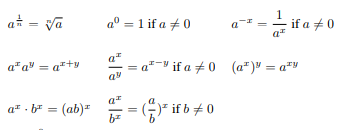
\includegraphics[scale = 1.0]{Graphics/Week_9/Exponent.PNG}
\end{center}
\section{Logarithm Laws}
If $a, x,$ and $y$ are non-zero real numbers, the rules for logarithms are:
\begin{center}
    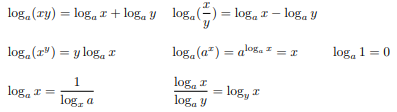
\includegraphics[scale = 1.0]{Graphics/Week_9/Log.PNG}
\end{center}
\section{Graph}
If $f(x) = a^x$ then $f^{-1}(x) = \log_ax$. The graphs of $f(x)$ and $f^{-1}(x)$ for $a = 2$ are shown below.
\begin{center}
    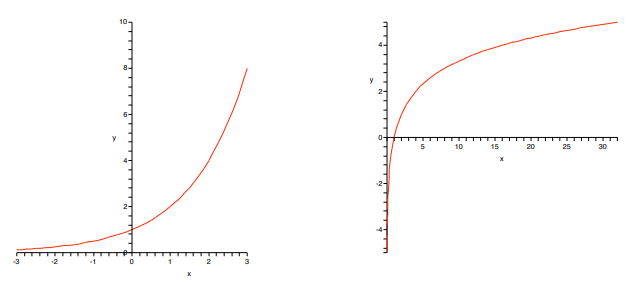
\includegraphics[scale = 1.0]{Graphics/Week_9/Graph.PNG}
\end{center}


\end{document}